%
% File acl2015.tex
%
% Contact: car@ir.hit.edu.cn, gdzhou@suda.edu.cn
%%
%% Based on the style files for ACL-2014, which were, in turn,
%% Based on the style files for ACL-2013, which were, in turn,
%% Based on the style files for ACL-2012, which were, in turn,
%% based on the style files for ACL-2011, which were, in turn, 
%% based on the style files for ACL-2010, which were, in turn, 
%% based on the style files for ACL-IJCNLP-2009, which were, in turn,
%% based on the style files for EACL-2009 and IJCNLP-2008...

%% Based on the style files for EACL 2006 by 
%%e.agirre@ehu.es or Sergi.Balari@uab.es
%% and that of ACL 08 by Joakim Nivre and Noah Smith

\documentclass[11pt]{article}
\usepackage{acl2015}
\usepackage{times}
\usepackage{url}
\usepackage{latexsym}
\usepackage{graphicx}
\usepackage{hyperref}
\usepackage[
    backend=biber,
    style=authoryear-icomp,
    natbib=true,
    url=false, 
    doi=true,
    eprint=false
]{biblatex}
\addbibresource{paper.bib}
\graphicspath{ {./figures/} }

%\setlength\titlebox{5cm}

% You can expand the titlebox if you need extra space
% to show all the authors. Please do not make the titlebox
% smaller than 5cm (the original size); we will check this
% in the camera-ready version and ask you to change it back.


\title{NLP Lab - Automated Journalist App}

\author{Ahmet Bilal Akın \\
  Technical University \\ of Munich \\
  {\tt bilal.akn@tum.de \\} \\\And
  Ecem Varma \\
  Technical University \\ of Munich \\
  {\tt ecem.varma@tum.de \\} \\\And
  Can Bilgin \\
  Technical University \\ of Munich \\
  {\tt bilgin@in.tum.de \\}}
  

\date{}

\begin{document}
\maketitle

\begin{abstract}
    To address the challenge of information overload from social media, we developed an Automated Journalist App that retrieves and summarizes social media content. The app incorporates advanced summarization techniques to provide both detailed insights and comparative analyses. This approach enhances user understanding by transforming raw social media data into actionable summaries, demonstrating the potential of automated content summarization to manage and interpret large volumes of information. In this paper, we also detail the technical implementation of the application, offering insights into the development and integration processes.
\end{abstract}

\section{Introduction}

In the era of information overload, social media platforms have become pivotal sources of real-time content, offering vast amounts of data that can be both overwhelming and challenging to interpret. To address this issue, we developed an Automated Journalist App, designed to streamline and distill social media feeds into meaningful summaries.

Our project aims to enhance the accessibility and comprehensibility of social media content by implementing advanced summarization techniques. The application retrieves data from various social media platforms and employs sophisticated natural language processing methods to generate concise and relevant summaries. This process includes two key summarization approaches: topic-aware summarization and delta summarization.

Topic-aware summarization involves generating summaries of the same content from multiple perspectives or topics, allowing users to gain insights into different aspects of the information presented. Delta summarization, on the other hand, facilitates a comparative analysis of summaries across different topics, highlighting the variations and similarities between them.

By integrating these techniques, our application not only provides users with streamlined content but also offers a nuanced understanding of the information through comparative analysis. This work aims to contribute to the field of automated content summarization by enhancing the utility and interpretability of social media data.

The Automated Journalist App is a group work of the authors of this paper. In the project, Can Bilgin was mainly responsible for selecting the technology stack, code quality, and software architecture. Furthermore, Can Bilgin implemented the communication between third-party social media platforms and our Automated Journalist App. Ecem Varma and Ahmet Bilal Akın worked together to conduct research and made decisions about which NLP techniques should be employed in this project. Alongside the research task, Ecem Varma had an active role in implementing the front end and Ahmet Bilal Akın was responsible for implementing the NLP techniques into the backend. However, this does not mean that we did distinct tasks and each person was only responsible for his/her section. Throughout the whole project, we exchanged our knowledge about the related topics and helped each other out while implementing our parts.  
\section{Related Work}\label{sec:related_work}
Automated journalism is an interesting concept that involves the use of machine learning models and natural language processing. It can simply be defined as automatically generating news content from a variety of resources. It's been already claimed that the use of automation in news creation is changing journalism (\cite{guzman2019prioritizing}) and it will continue to do so. Here, we would like to discuss some of the prominent automated journalism applications that we find worth mentioning.
\subsection{Bloomberg’s Cyborg}
Bloomberg uses an application called Cyborg to help reporters with their financial reports about company earnings. This helps Bloomberg's journalists to create more complex financial articles (\cite{micklethwait2018future}). It creates news stories from a vast amount of financial articles and displays an overview.
\subsection{WordSmith by Associated Press (AP)}
AP uses Wordsmith to automatically generate earnings reports for various companies. Rather than manually extracting information from the financial reports quarterly released by the companies, it allows journalists or reporters to access well-structured and readable texts. In other words, WordSmith extracts the financial data and generates reports that sound fluent and plausible.
\subsection{Reuters News Tracer}
This tool helps Reuters journalists detect and verify newsworthy events on Twitter in real-time. In other words, it performs event detection using clustering to find more prominent events. Moreover, to determine which events are more newsworthy than others, it leverages a ranking algorithm. In addition, it's able to update the summaries based on the changing events in a time period, i.e., it has the ability to perform temporal summarization. Since working with social media data is relatively harder than structured reports or articles, we think Reuters News Tracer is an impressive real-time application.
\subsection{Quakebot by the Los Angeles Times}
The last application that draws our attention is Quakebot\footnote{\href{https://www.latimes.com/people/quakebot}{Quakebot, https://www.latimes.com/people/quakebot}}. It is a software application that reports the latest earthquakes using data from the U.S. Geological Survey. Its relation with automated journalism is it generates a draft article if the earthquake notices are above a certain threshold. It's reviewed by an editor and published if it's found newsworthy.
\section{Implementation and Technologies}\label{sec:technology}

We have developed the Automated Journalist App using appropriate technologies. To meet our requirements, we needed a user-friendly application with a modern design, supported by a frontend framework that aligns with our design concept. In addition, before starting the project we had a codebase written in Python capable of generating summaries from given texts. Our objective was to extend this codebase, integrate it with a user interface, and transform it into a fully functional application. We carefully selected our technology stack to align with these goals.

Furthermore, we integrated two additional APIs into the application alongside the Twitter API. Specifically, we implemented connections to Reddit and Telegram, enabling us to use these platforms as additional data sources. 

The technologies we selected for this app are:
\begin{itemize}
    \item Backend: Python with Flask Framework
    \item Frontend: React with Typescript
    \item UI/UX design: Figma
\end{itemize}

The structure of the application is as in the following diagram (figure \ref{fig:architecture}). As illustrated in the figure, the Flask application serves as the bridge between the frontend, third-party social media APIs, and our AI models, which are used to summarize content from the social media feeds.

\begin{figure}
    \centering
    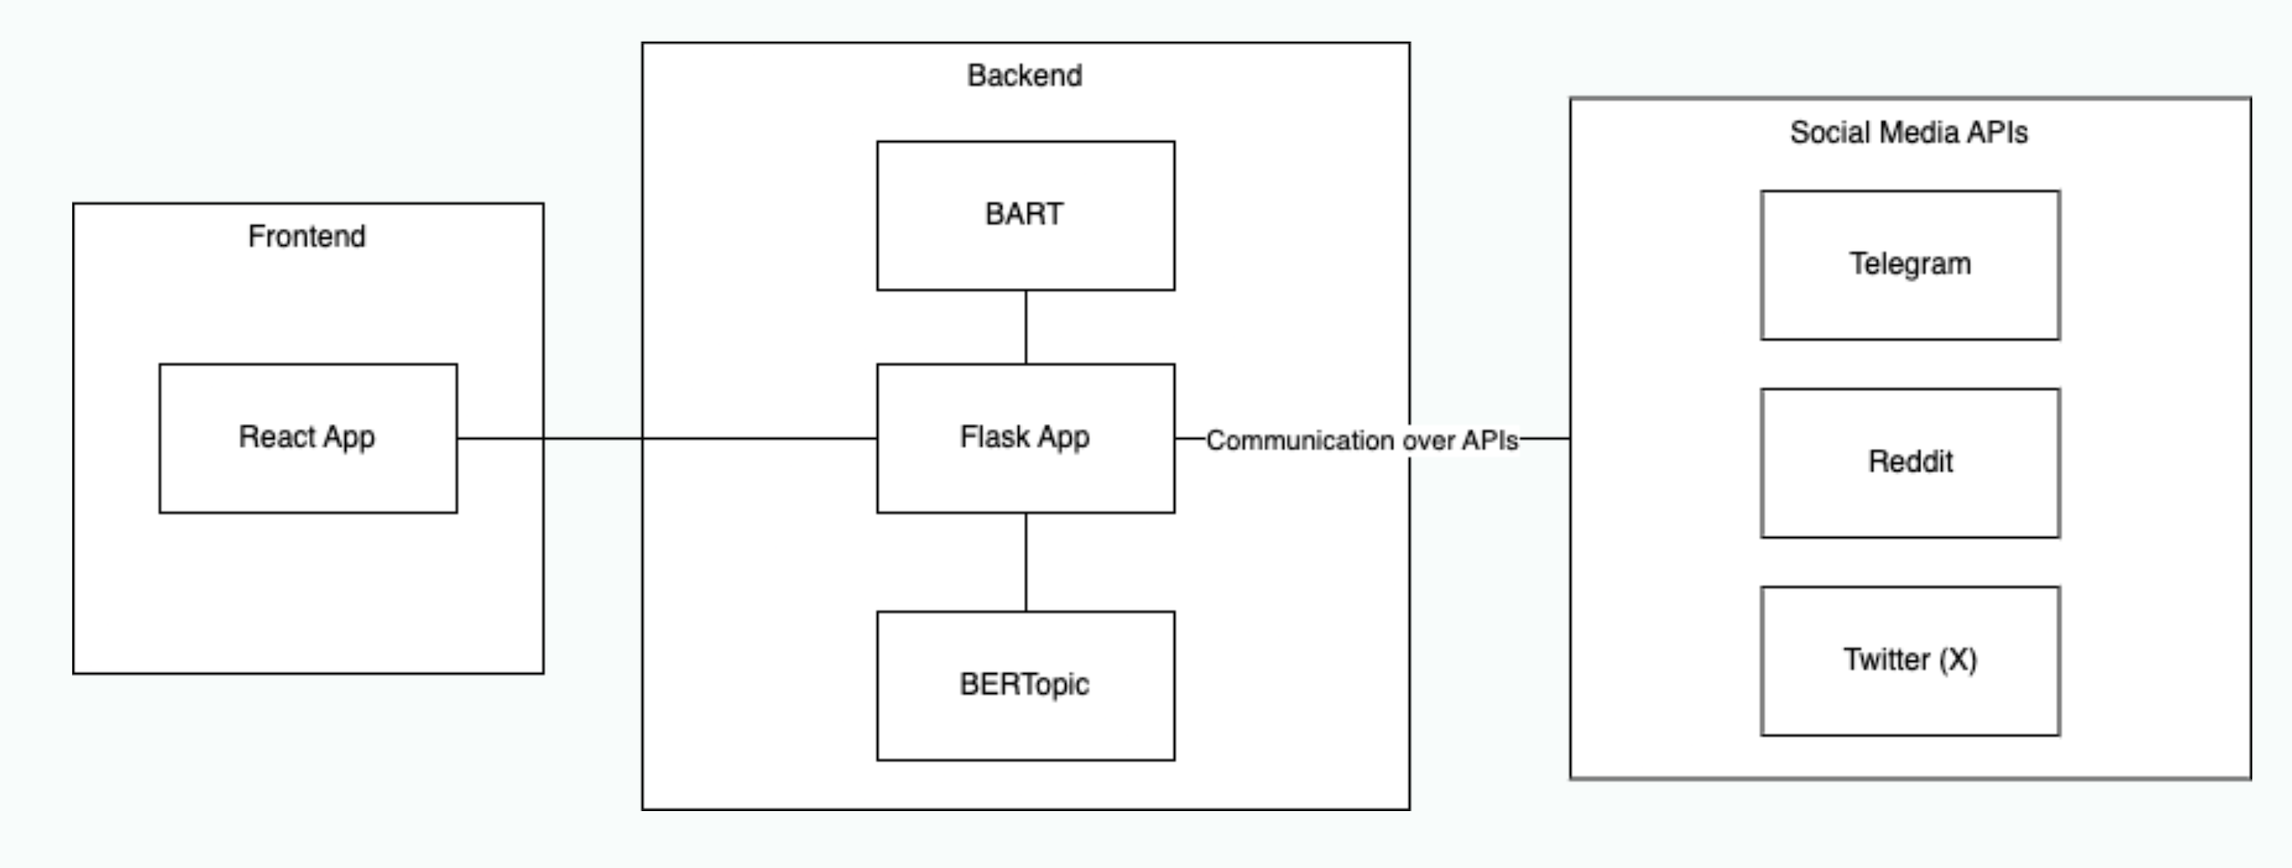
\includegraphics[width=\linewidth]{figures/general-architecture-of-the-app.png}
    \caption{Architecture of the App}
    \label{fig:architecture}
\end{figure}

\subsection{Backend}

As previously mentioned, at the outset of the project, we had a Python codebase as our starting point. We extended this code to develop the project into a fully functional application. Python was also chosen due to its extensive libraries, which are particularly advantageous in the fields of machine learning and natural language processing.\citep{ml-python}

Moreover, Python offers several libraries that facilitate the integration of third-party applications through their APIs. Relevant examples include Twat for Twitter, PRAW for Reddit, and Telethon for Telegram.

The backend application functions as a REST API endpoint for the frontend, and it is built using Python Flask. This Flask application consolidates calls to third-party APIs and integrates them with the NLP models we use for generating summaries. The application does not include any authentication or authorization mechanisms. The social media feeds obtained from the sources are not personalized; rather, they are retrieved by querying these platforms through the API endpoints maintained and published by the respective social media providers. At the backend application, we implemented some endpoints only retrieving data from the respective social media platforms.

Additionally, we have implemented endpoints to process summaries from the feeds selected by the user. Our application offers three distinct summarization functionalities: "Default Summary," "Topic-Aware Summary," and "Delta Summary."
\begin{itemize}
    \item The Default Summary provides a summary of the selected feed.
    \item The Topic-Aware Summary generates potential topics from the default summary and then produces summaries of the same feed, tailored to those identified topics.
    \item The Delta Summary allows users to compare summaries across different topics, enabling them to see how divergent the summaries are within various topic perspectives.
\end{itemize}

Details on the specific implementation of these functionalities, including the models used, will be provided in the section \ref{sec:summarization} "Summarization Techniques".

\subsection{Frontend}
To enable access to the application's functionalities, we have implemented a web-based user interface. For the user interface, we utilized the React framework with TypeScript, which provided the advantage of using hooks to create a more responsive application with improved communication between the frontend and backend. While implementing the application, we have tried to utilize the principles of Object Oriented Programming.

Before writing any code, we first created a design concept using Figma. Once the concept was established, we began coding. During the development process, we made extensive use of the React library Material-UI to align the implementation with our design as closely as possible.

\subsection{Samsum Dataset Format}\label{subsec:samsum}

In our application, we retrieve data from various social media providers and needed to standardize this data into a uniform format. This standardization ensures that our summarization implementation can effectively process and summarize data across different social media platforms. To achieve that goal, we utilized the "Samsum Dataset Format" which was introduced by \cite{samsum}. We fetched that data from the social media and transformed the data with the following schema:
\begin{itemize}
    \item dialogue: text of dialogue.
    \item summary: human written summary of the dialogue.
    \item id: unique id of an example.
\end{itemize}

We have also utilized this format as an interface between the backend and frontend. The application fetches data from a social media platform and sends it to the frontend as in the defined "samsum" format. The social media feed is then displayed accordingly. When a user wishes to summarize a feed, they select the feed by clicking on it. The selected feed is then transmitted in the "samsum" format to the backend, where it is summarized. This methodology streamlines the process of handling data from different sources, as it eliminates the need to format each source individually. Moreover, if there is a need to integrate additional data sources, the same methodology can be employed. The new feed can be converted to the "samsum" format, allowing the existing functionalities to be applied seamlessly.
 
\subsection{How does the application work?}\label{subsec:how_app_work}
This subsection outlines how the application functions from a user's perspective. We will explore the actual use cases of the application, accompanied by real in-app screenshots, to provide a clearer understanding of how the app operates. The in-app screenshots are given at the end of the report in Appendix \ref{sec:appendix}.

The application does not include any authorization or authentication mechanisms as also stated above. As a result, when the user accesses the home page, they can immediately begin using the application's functionalities without the need for any additional steps.

The home page of the application greets the user with a search bar, allowing them to perform queries within social media platforms. Above the search bar, there are tabs where the user can select the specific social media provider from which the query will be issued. The screenshot of the displayed figure has been given in the Appendix as the figure~\ref{fig:home_page}.

Once the feeds are fetched from the social media, they are displayed to the user. A feed is a set of data that is structured as in the samsum dataset format as also described in the subsection "Samsum Dataset Format" (Section \ref{subsec:samsum}). Some conversations in the social media have been displayed to the user as in the figure \ref{fig:home_page}

The user then selects one of these conversations, which is sent to the backend for summarization. Upon completion of the summarization task, the "Default Summary" is returned and displayed to the user. Simultaneously, the "Topic-Aware Summary" is processed, along with the associated topics. These topics are also presented in the user interface. To view summaries related to each specific topic, the user can select the desired topics from a drop-down menu located at the top right of the display, as shown in the figure \ref{fig:summary_default}.

Subsequently, the user selects a topic from the drop-down menu, and the summary related to that topic is displayed (see figure \ref{fig:summary_topic_options}). Additionally, the user can compare summaries across different topics to assess how they differ from one another. To utilize this functionality, the user clicks the "Compare Summaries" button, which opens a selection popup. The user then selects the topics to be compared.(figure \ref{fig:compare-summaries})

Once the topics are selected, these choices are transmitted to the backend to generate the "Delta Summary." The results of the "Delta Summary" are presented in two visualization formats: a scatter plot (figure \ref{fig:delta-summary-scatter}) and a cosine similarity matrix (figure \ref{fig:delta-summary-cosine}).
\section{Summarization Techniques}\label{sec:summarization}
In this section, we review the summarization techniques utilized in our application. As it's mentioned in section \ref{sec:technology}, we already had an application capable of creating summaries. The main contribution made by our group is extending the summary capabilities with topic-aware summarization and delta summarization. \\
To have a basic understanding of how summarization is made in our application, we should start explaining the existing model and how we utilized it. Although the summarization model can be configured via a configuration file, we used "philschmid/bart-large-cnn-samsum" from Hugging Face (\cite{schmid2021bart}). This model is pre-trained with the samsum dataset (\cite{samsum}). Since it contains several conversations and their respective summaries, the pre-trained model matched our objectives. We knew that BART has some limitations such as the token limit of 1024 but decided to use it as the main focus of this project is integrating the topic-aware summarization and delta summarization modules. To overcome the maximum token limit problem, we leverage chunking to split the text into smaller pieces. By having different text pieces with smaller sizes, our BART model is capable of producing a summary from those. In other words, the overall summary consists of the summaries generated from the chunked parts.
\subsection{Topic-Aware Summarization}
Topic modeling was one of the already implemented features in our app. Therefore, we could extract the topics from a given set of documents. Our first approach is using the conversations streamed from Reddit and Telegram and feed them as documents to our BERTopic \footnote{\href{https://maartengr.github.io/BERTopic/index.html}{BERTopic, https://maartengr.github.io/BERTopic/index.html}} model. Since we did not have the API implementations in the first place, the Samsum dataset was used for the conversation data. Topic-aware summarization flow can be described as the following:
\begin{itemize}
    \item Extract topics and respective topic embeddings from the streamed conversations utilizing BERTopic.
    \item Extract sentences from the dialogue to be summarized with respect to a similarity score. Here, we use a sentence transformer, "paraphrase-multilingual-MiniLM-L12-v2" (\cite{reimers-2019-sentence-bert}), from Hugging Face to create the embeddings of the sentences. By comparing the sentence embeddings of the dialogue with the topic embeddings, a similarity matrix is generated. Each sentence is mapped to the most similar topic, and, eventually, for each topic (potentially) we have some extracted sentences.
    \item Finally, we have extracted sentences for each topic and as a final layer, they feed into our BART summarizer model for abstractive summarization.
\end{itemize}
One major challenge we face is the lack of conversations fetched from the APIs. Since our app is available in English, we filtered out the conversations in different languages. This created a bottleneck in the usage of BERTopic because it requires a minimum number of documents to generate a meaningful output. As a fallback mechanism, we introduced static pre-defined topics. If BERTopic fails to create the topics, we use static topics and their embeddings to create the topic-aware summarizations.
\subsection{Delta Summarization}
Delta summarization may sound misleading in the context of our application as we do not create a summary but a comparison. The main idea is to compare two different topic summaries and visualize them in a certain format. The currently supported formats are cosine similarity matrices and scatter plots (2D).
\subsubsection{Cosine Similarity Matrix}
It's a matrix where the items are cosine similarity values of the two respective topic summaries. We first find the cosine similarity value between two summaries by using their sentence embeddings. The sentence encoder, "all-MiniLM-L6-v2", is utilized to create those embeddings. It's a pre-trained model from Hugging Face and is from the sentence-transformers family. After having the cosine similarity values, we create the matrix as an output (\ref{fig:delta-summary-cosine}).
\subsubsection{Scatter Plot}
To create this format, we follow a common approach. That is, we create the sentence embeddings as it's been done in the cosine similarity matrix. Having this, Principal Component Analysis (PCA) is applied for dimensionality reduction to the high-dimensional embeddings. In other words, sentence embeddings created by the sentence transformer have 384 dimensions and to be able to show it in a 2D plot, we must apply a dimensionality reduction technique. PCA is selected because it's easily applicable from open-source libraries and is also a well-known method. After all, we see a 2D scatter plot showing how similar the two summaries are (\ref{fig:delta-summary-scatter}). This is helpful since we can observe the similarity of different topic summaries and also compare them with the original dialogue and the default summary.
\section{Challenges}\label{sec:challenges}

During the development of the Automated Journalist App, we encountered several challenges that required adaptive solutions:

1. Transition from Twitter API: Initially, our project relied on the Twitter API for data retrieval. However, when Twitter's API transitioned to a paid model, we had to change it. To maintain the project's scope, we integrated alternative APIs from platforms like Reddit and Telegram. This shift necessitated modifications in our data processing pipeline to accommodate the different structures and content types provided by these platforms.

2. Limitations of BERTopic: We employed BERTopic to extract topics from input texts, which generally provided valuable insights. However, the model struggled when working with shorter texts, often failing to generate meaningful topics. To address this, we implemented a fallback mechanism using a predefined list of topics, ensuring that even brief inputs could be categorized effectively. Also in cases where the text is long enough, the topics BERTopic produced were not entirely meaningful.

3.	Slowness in Summarization: The summarization process using the BART model was slower than anticipated. This slowness affected the responsiveness of the application.
\section{Results}\label{sec:results}

The Automated Journalist App achieved its goal of streamlining and summarizing social media content from multiple platforms. Through the integration of Reddit and Telegram APIs, the application was able to retrieve and process data from diverse sources, ensuring a broad coverage of social media conversations.

Topic Extraction and Summarization:
\begin{itemize}
    \item The use of BERTopic for topic extraction provided valuable insights into the data, allowing for the identification of key themes within the social media feeds. Although there were challenges with shorter texts, the fallback to predefined topics ensured that the application consistently delivered relevant categorizations.
\end{itemize}
\begin{itemize}
    \item The BART model for summarization effectively condensed social media feeds into coherent summaries. Despite some performance bottlenecks, the summaries were meaningful and coherent.
\end{itemize}

User Interface and Experience:
\begin{itemize}
    \item The web-based user interface, implemented with React and TypeScript is easy to use. The integration of Material-UI components gives the application a modern and intuitive design, enabling users to quickly access and navigate through the app's features.
\end{itemize}
\begin{itemize}
    \item The implementation of Topic-Aware Summaries and Delta Summaries added depth to the user experience by allowing users to explore different perspectives and compare topic-based summaries.
\end{itemize}

In summary, the Automated Journalist App effectively addressed the challenge of information overload on social media by providing good quality, automated summaries. The results validate the application's approach and highlight its potential for further development and refinement.

\section{Discussion and Future Work}\label{sec:discussion}
One of the primary challenges we encountered was the application's performance. While effective in generating adequate quality summaries, the BART model introduced latency issues that impacted the user experience. This raises a problem with the app's responsiveness. Exploring more efficient models or optimizing the existing implementation might help strike a better balance.

One promising direction is the exploration of the Flan-T5 model for topic modeling. Flan-T5, known for its strong performance in various natural language processing tasks, could potentially offer more accurate and contextually relevant topic extraction, even for shorter texts. Fine-tuning Flan-T5 specifically for the task of topic modeling might address some of the limitations we encountered with BERTopic, particularly in generating meaningful topics from minimal input.

For the summarization task, several models could be considered to improve both the quality and speed of the generated summaries. The Flan-T5 model, when fine-tuned for summarization, could offer a powerful alternative to the BART model, potentially delivering faster processing times without compromising the quality of the summaries. Additionally, Pegasus, a model pre-trained specifically for abstractive summarization, could be another viable option. Pegasus is designed to handle summarization tasks effectively and might yield more concise and coherent summaries.

Moreover, the use of large language models (LLMs), such as GPT-4 or similar advanced models, could further enhance the summarization capabilities. These models have demonstrated exceptional performance in generating human-like text and could provide summaries that are not only accurate but also nuanced and contextually rich. However, integrating LLMs would require careful consideration of computational resources and cost, as well as strategies to mitigate potential biases in the generated content.\citep{shakil2024evaluating}

The limitations of BERTopic in processing shorter texts highlighted a significant challenge in natural language processing: extracting meaningful information from minimal input. Our fallback solution of using predefined topics was a practical response, but it also introduced a degree of inflexibility. In future work, incorporating techniques that can adaptively enhance the context or dynamically adjust the topic modeling process for shorter texts could improve the robustness of the application.

For the user interface, it can be more intuitive and responsive. Future work could explore more advanced UX/UI features, such as more sophisticated visualization tools, or even personalized summarization based on user preferences.

As the app evolves, scalability will become an increasingly important factor. Expanding the app to handle larger volumes of data or integrating it with more platforms will require careful infrastructure and software architecture planning. Additionally, the potential applications of the app extend beyond journalism; it could be adapted for use in various industries, such as market research, public relations, or any field that requires real-time analysis of social media content.

\section{Conclusion}\label{sec:conclusion}
In this lab course, we integrated several new functionalities into an existing end-to-end application. The most prominent features are the integration of Telegram and Reddit APIs, topic-aware summarization, and delta summarization. Furthermore, since those implementations can not be grasped easily without meaningful visuals, we build a user interface in the form of a React application. We believe this makes it easier for users to navigate and interact with the system. \\
To conclude, our main contributions to the automated journalist application are integrating the social media APIs, topic-aware and delta summarization, and implementing a front-end application. With these, we extended the features of an existing end-to-end application and developed a user interface from scratch. 

\printbibliography 

\onecolumn
\appendix
\section{Appendix}\label{sec:appendix}

\clearpage


\begin{figure}
    \centering
    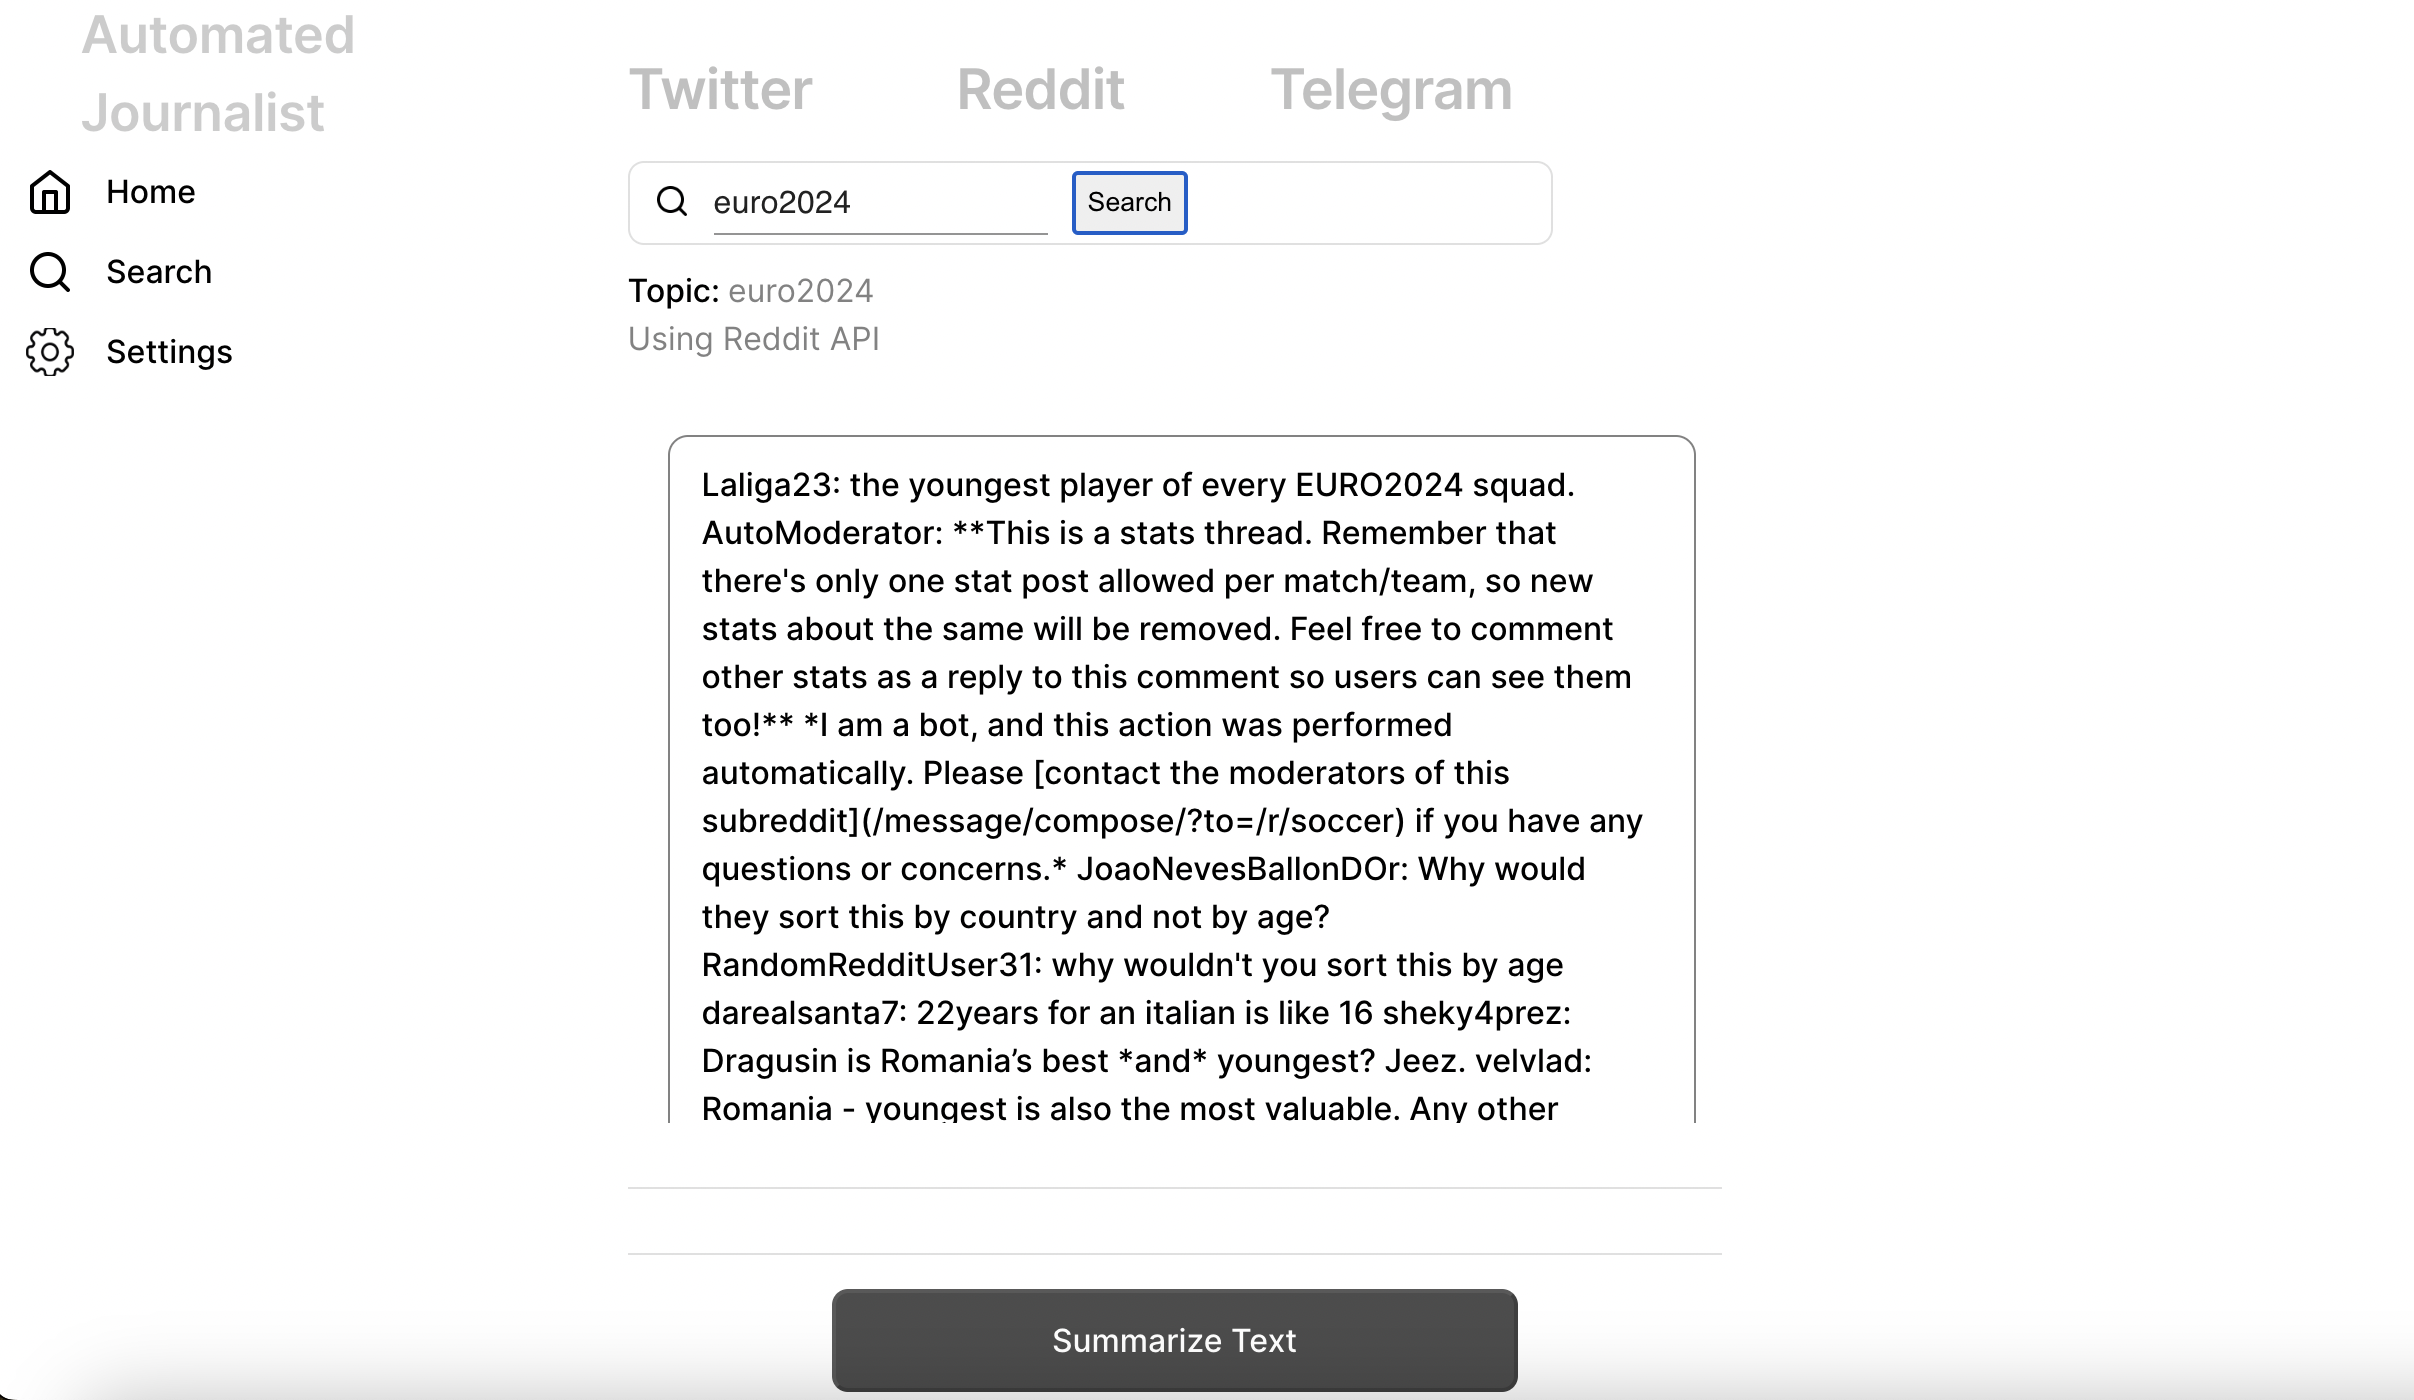
\includegraphics[width=\linewidth]{figures/inside-app-screen-shots/query-search.png}
    \caption{Home Page}
    \label{fig:home_page}
\end{figure}

\begin{figure}
    \centering
    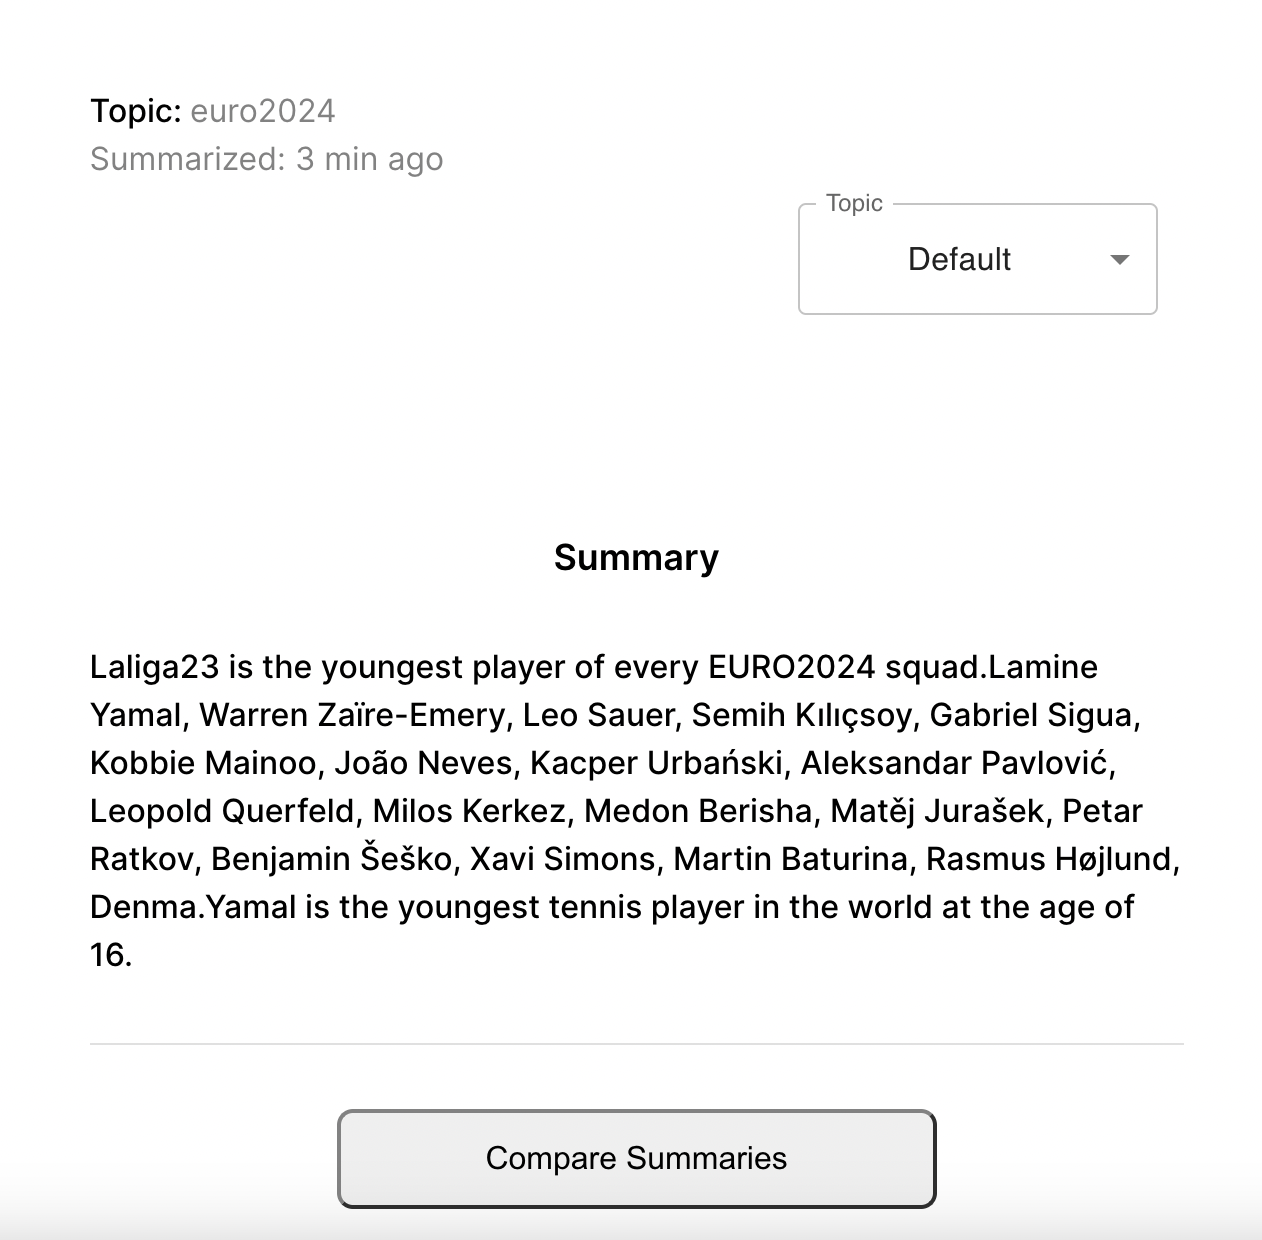
\includegraphics[width=\linewidth]{figures/inside-app-screen-shots/summary-default.png}
    \caption{Default Summary}
    \label{fig:summary_default}
\end{figure}


\begin{figure}
    \centering
    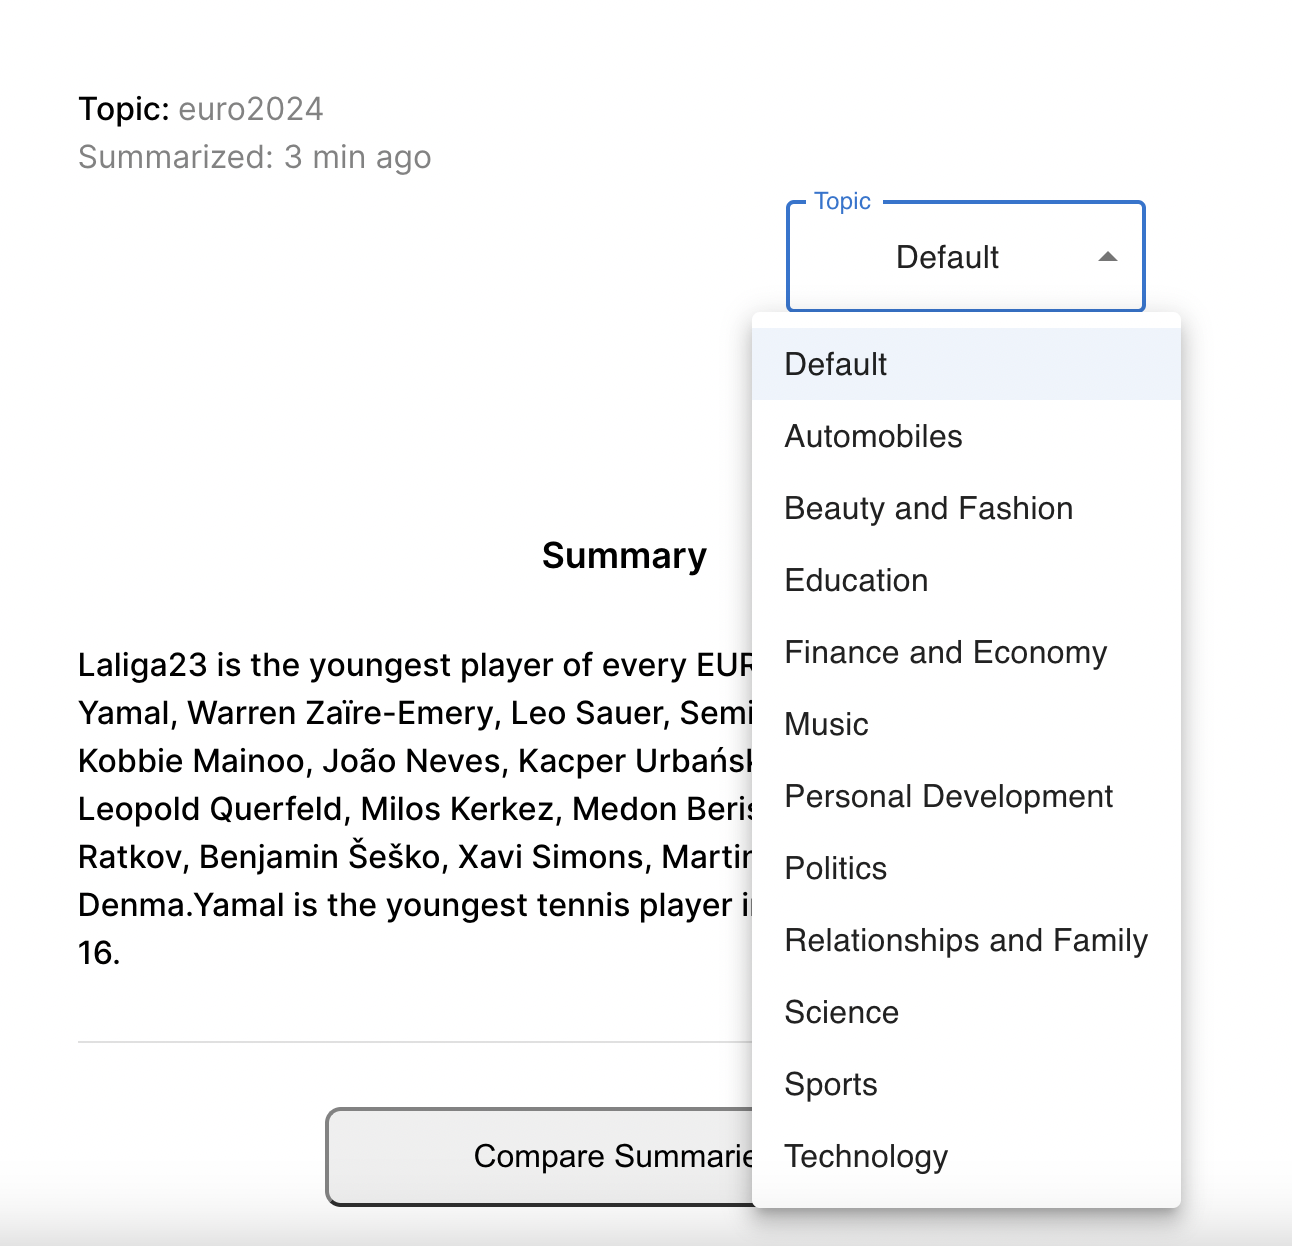
\includegraphics[width=\linewidth]{figures/inside-app-screen-shots/summary-topic-options.png}
    \caption{Topics Aware Summary}
    \label{fig:summary_topic_options}
\end{figure}


\begin{figure}
    \centering
    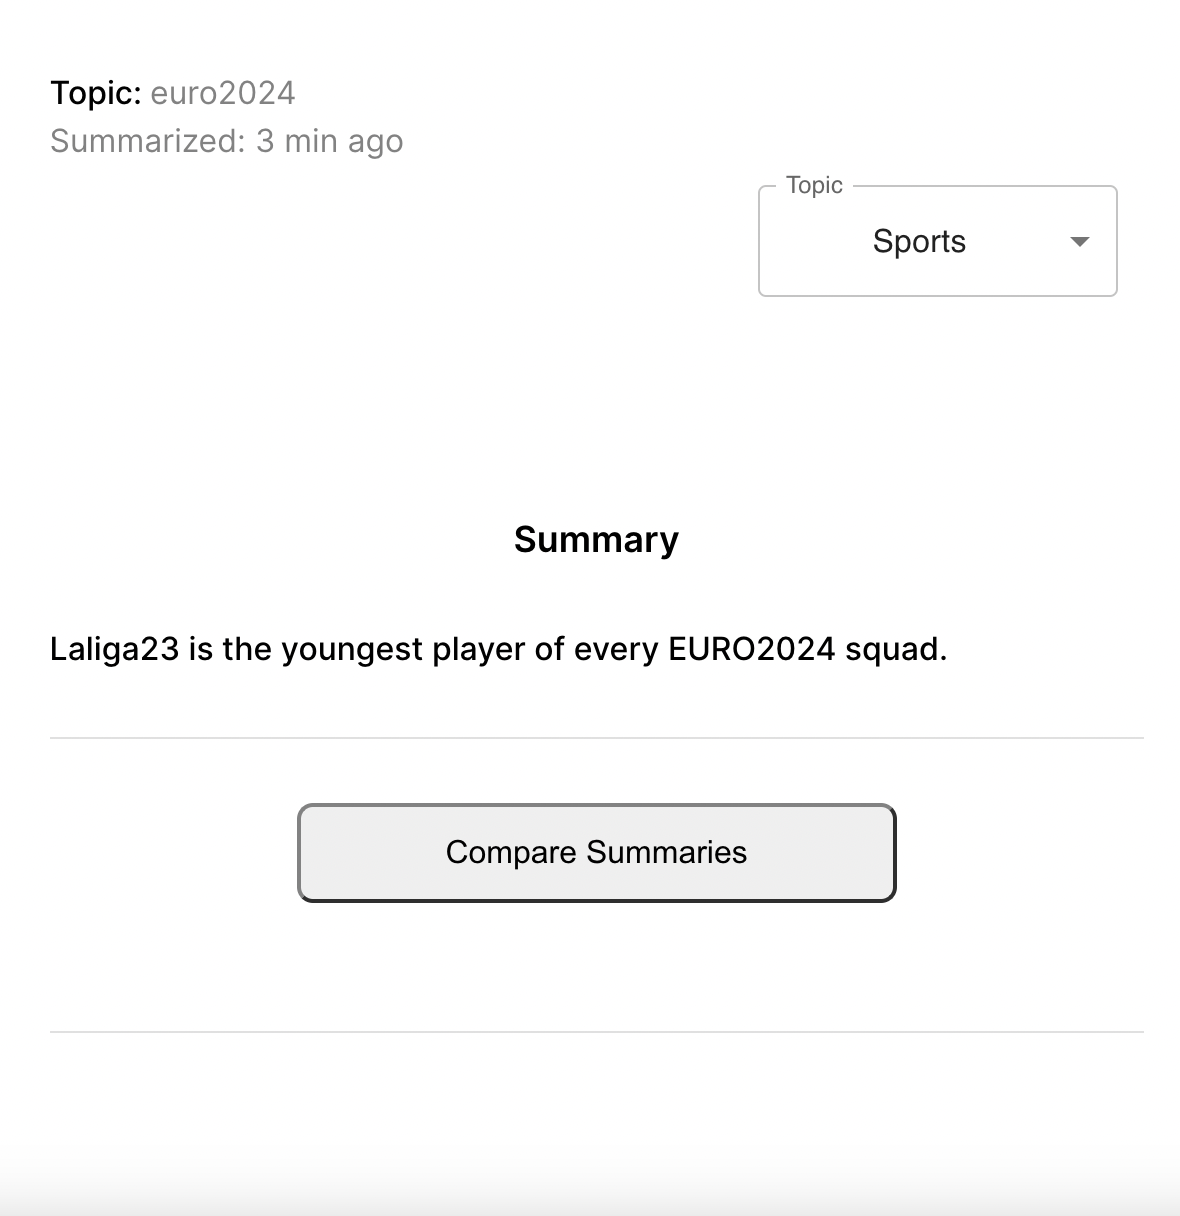
\includegraphics[width=\linewidth]{figures/inside-app-screen-shots/summary-sports.png}
    \caption{Example Topic: Sports}
    \label{fig:summary-sports}
\end{figure}


\begin{figure}
    \centering
    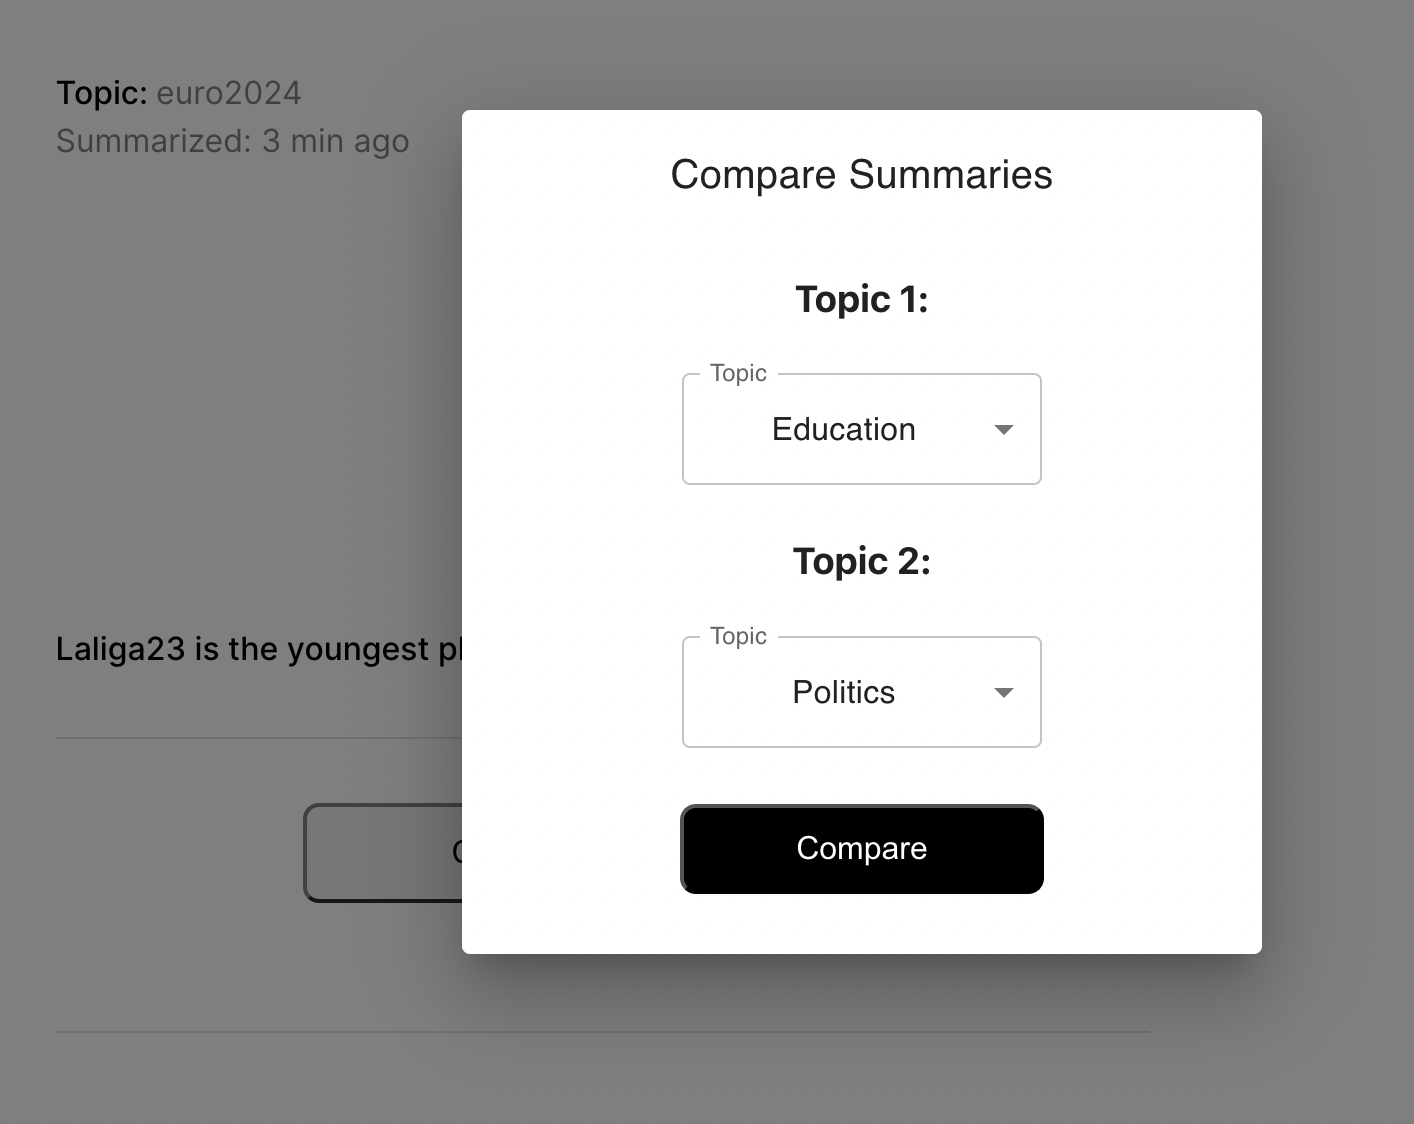
\includegraphics[width=\linewidth]{figures/inside-app-screen-shots/compare-summaries.png}
    \caption{Delta Summary Options}
    \label{fig:compare-summaries}
\end{figure}

\begin{figure}
    \centering
    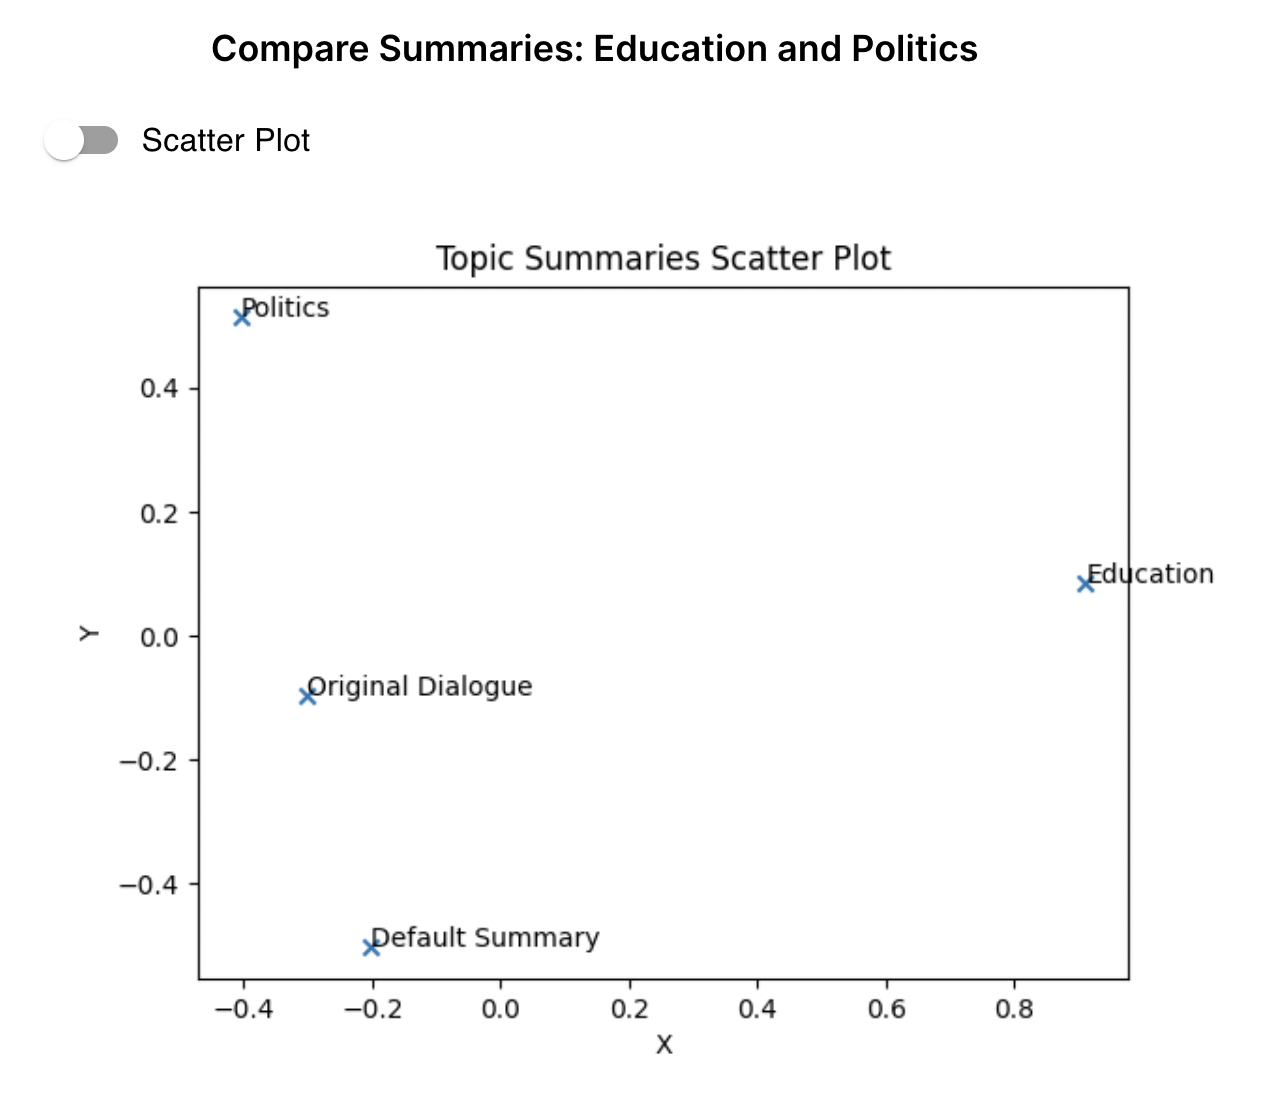
\includegraphics[width=\linewidth]{figures/inside-app-screen-shots/delta-summary-scatter.png}
    \caption{Delta Summary: Scatter Plot}
    \label{fig:delta-summary-scatter}
\end{figure}

\begin{figure}
    \centering
    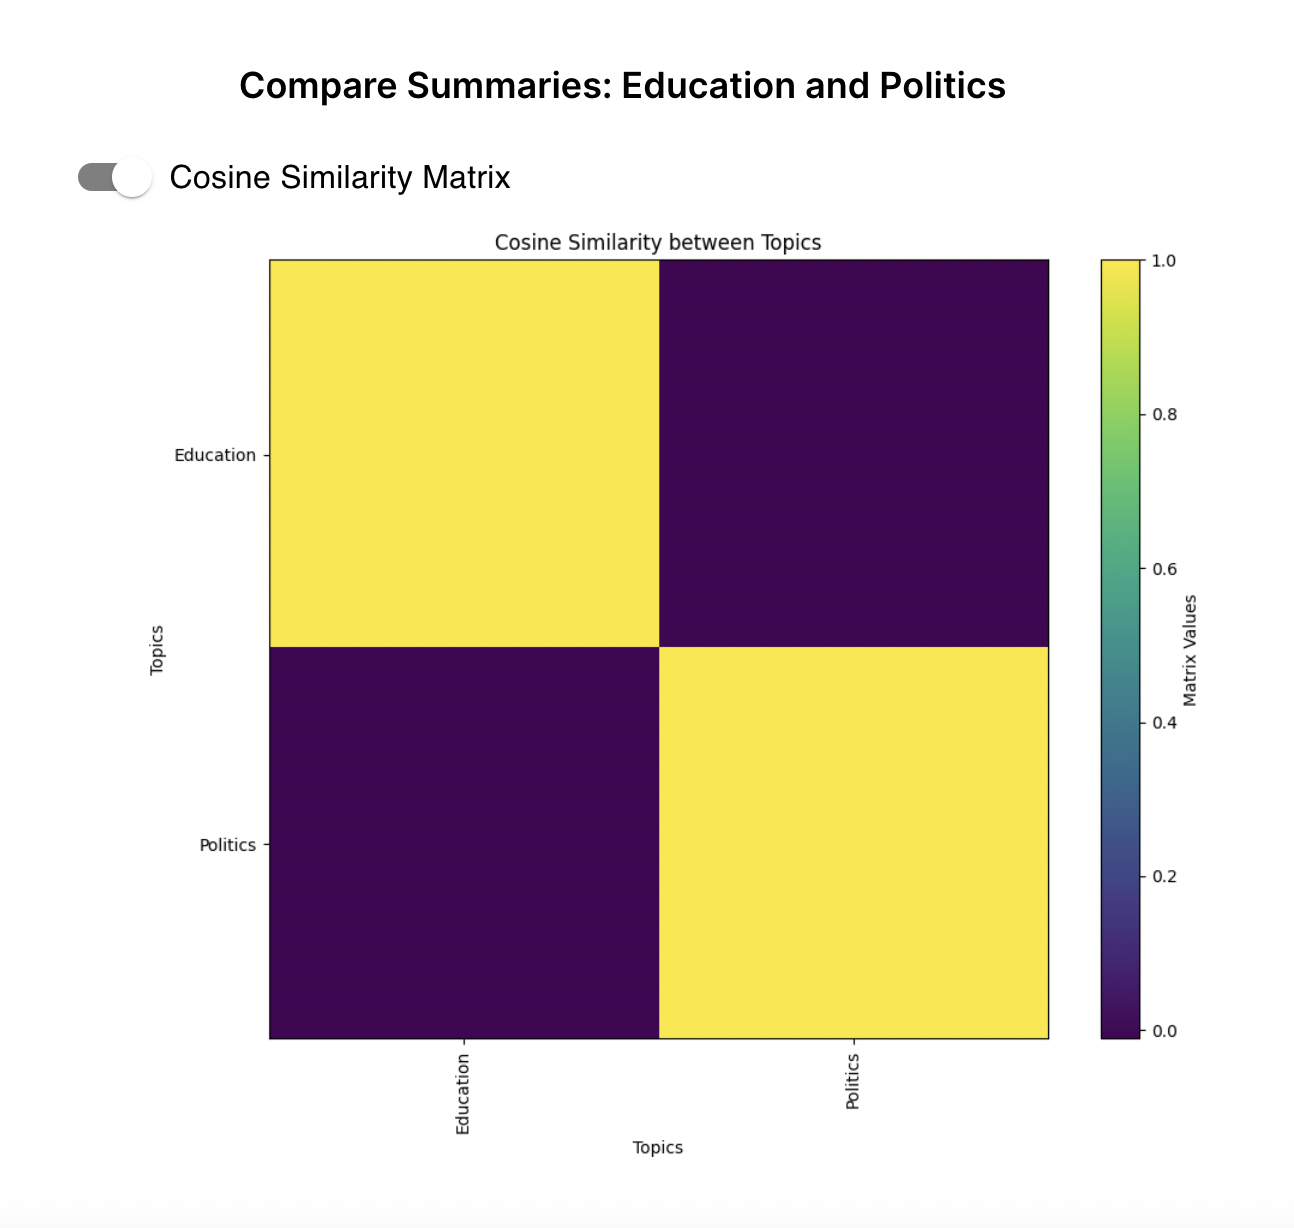
\includegraphics[width=\linewidth]{figures/inside-app-screen-shots/delta-summary-cosine.png}
    \caption{Delta Summary: Cosine Similarity Matrix}
    \label{fig:delta-summary-cosine}
\end{figure}














\end{document}